\documentclass[12pt,fleqn]{article}
\setlength{\parindent}{0pt}
\usepackage{graphicx}
\usepackage{cancel}
\usepackage{listings}
\usepackage[latin5]{inputenc}
\usepackage{color}
\setlength{\parskip}{8pt}
\setlength{\parsep}{0pt}
\setlength{\headsep}{0pt}
\setlength{\topskip}{0pt}
\setlength{\topmargin}{0pt}
\setlength{\topsep}{0pt}
\setlength{\partopsep}{0pt}
\setlength{\mathindent}{0cm}
\usepackage{latexsym}
\usepackage{amsfonts}
\usepackage{showkeys}
\renewcommand*\showkeyslabelformat[1]{(#1)}

\begin{document}
Ders 1 

Diziler (Sequences)

Bir dizi aslinda sadece bir listedir. Listede 1. eleman vardir, 2. eleman
vardir, vs. ve bu sonsuza kadar devam eder. Bu nokta onemli, matematikte
sonlu / sinirli (finite) bir liste dizi degildir. Dizilerin onemli bir
ozelligi sonsuza kadar devam etmeleridir. 

Daha formel olarak bakarsak dogal sayilarin, yani $\mathbb{N}$ kumesinin de
tanimda bir rol oynadigini gorebiliriz. Listedeki her eleman dizideki sira
numarasi ile etiketlenebilir, 1. elemani ``1'', 2. elemani ``2'',
vs. olarak etiketleyebiliriz, o zaman bu acidan bakarsak bir dizinin, dogal
sayilar ile baska bir kume arasindaki bir {\em eslesme} oldugunu da
soyleyebiliriz. Bu eslesme bir diger tanimla bir fonksiyondur. Yani bir
dizi aslinda bir fonksiyondur, yani 

\[ f: \mathbb{N} \to \mathbb{R} \]

Dizimizi 

\[ f(1),f(2),f(3),...,f(n),.. \]

olarak gosterebiliriz. 

Yaklasmak (Convergence) 

Acik bir sekilde gorulecegi uzere alttaki dizi

\[ 1,\frac{1}{2},\frac{1}{3},\frac{1}{4},... \]

gittikce 0 degerine dogru gidiyor. Bu dizi ``sifira yaklasiyor
(convergence)'' deriz, ya da ``dizinin limiti sifir'' deriz. Peki bu fikri
nasil daha acik, net olarak tanimlayabiliriz? 

Yaklasan seriler 18. yuzyilda incelendi ve gelistirildi, fakat o zamanlarda
bu tur dizilerin tanimi hicbir net olarak ortaya koyulmadi. Literatur
taranirsa tanima en yakin olacak sey soyledir:

``Bir dizi $\{s_n\}$ $L$ sayisina yaklasir, eger bu dizideki terimler
gittikce $L$'e yakinlasliyorsa''. 

Bu tanimin oldukca genel, kabaca olarak yapilmis olmasi bir yana, bazen
bizi yanlis yollara bile surukleyebilir. Mesela su diziyi ele alalim 

\[ .1, .01, .02, .001, .002, .0001, .0002, .00001, .00002, ... \]

Bu dizi muhakkak sifira ``yakinlasiyor'', fakat terimler duzenli bir sekilde
sifira yaklasmiyorlar. Her ikinci adimda birazcik sapiyorlar. Ya da su dizi

\[ .1, .11, .111, .1111, .11111, .111111, ... \]

Bu dizi gittikce .2'ye ``yakinlasiyor'', fakat bu dizinin .2'ye yaklastigi
iddia edilemez. Gercek limit 1.9 olmali, 2 degil. Ne oldugu belli olmayan
bir ``gittikce yaklasma'' tanimina degil, bizim aslinda ``gelisiguzel
yakinlik (arbitrarily close)'' tanimina ihtiyacimiz var.

Bu fikri en iyi yakalayabilen 1820'li yillarda Augustin Cauchy
oldu. Esitsizlikleri kullanarak ``herhangi / gelisiguzel yakinlik''
kavramini formule eden bir tanim bulmayi basardi. Bu sekilde limit kavrami
gayet acik matematiksel esitliszlikler ile gosterilebildi.

Tanim: Bir Dizinin Limiti 

$\{s_n\}$'nin reel sayilardan mutesekkil bir dizi oldugunu
dusunelim. $\{s_n\}$'nin bir reel sayi $L$'e yaklastigini soyleriz, ve bunu

\[ \lim_{n\to\infty} s_n = L \]

olarak belirtiriz. Ya da

\[ s_n \to L \ olur, \ n \to \infty \ iken \]

eger her $\epsilon > 0$ icin oyle bir tam sayi $N$ var ise, ki bu $N$ su
sartlara uymali

\[ |s_n - L| < \epsilon  \]

$n \ge N$ oldugu her zaman icin. 

Bir dizi yaklasmiyorsa, ona uzaklasan (divergent) dizi adi verilir. Bu her
iki tur ile ayni derecede ilgileniyoruz. 

Not: Tanimda $N$'nin $\epsilon$'a bagli oldugu goruluyor, eger $\epsilon$
cok ufak ise mesela, o zaman $N$'in oldukca buyuk olmasi
gerekebilir. Bu acidan bakilinca aslinda $N$'nin $\epsilon$'nun bir
fonksiyonu oldugu soylenebilir. Bu durumu tam vurgulamak icin bazen
$N(\epsilon)$ yazmak daha iyi olabilir. 

Not: Tanima dikkat edersek, sartlara uyan bir $N$ bulununca, o $N$
degerinden daha buyuk herhangi bir $N$ de kullanabiliriz. Yani ustteki
tanim bize herhangi bir $N$ bulmamizi soyler, illa ki ``en kucuk'' $N$'i
bulmamiz gerekmez. 

Tanim bunu soylemiyor olsa bile ibarenin asil gucu $N$'nin {\em $\epsilon$
  ne kadar kucuk olursa olsun bulunabiliyor olmasidir}. Eger $\epsilon$
buyuk bir sayi ise $N$'i bulmak kolay olur. Eger $\epsilon = 0.1$ icin (ki
bu sayi $\epsilon$ turu sayilar icin buyuk sayilir) isleyen bir $N$
bulursak, ayni $N$ daha buyuk  $\epsilon$ degerleri icin de isleyecektir. 

Ornek 

Ustteki tanimi kullanarak 

\[ \lim_{n \to \infty } \frac{n^2}{2n^2 + 1} = \frac{1}{2} \]

oldugunu ispat edelim. Yanliz sunu belirtelim, ustteki tanim limitin 1/2
olacagini hesaplamak teknigi olarak verilmiyor. Ifade limit kavramina kesin
bir tanim getiriyor ama o limiti hesaplamak icin kesin bir metot
sunmuyor. Neyse ki cogumuz bu hesabi yapmak icin yeterince calculus
hatirliyoruz, boylece limitin dogrulugunu ispatlamadan once ne oldugunu
bulabiliriz.

\[ \lim_{n \to \infty } \frac{n^2}{2n^2 + 1}  =
\lim_{n \to \infty } \frac{1}{2 + 1/n^2} =
\frac{1}{\lim_{n \to \infty }(2 + 1/n^2)} 
\]

\[ = \frac{1}{2 + \lim_{n \to \infty }(1/n^2)}  = \frac{1}{2} \]

Bu hesap, eger tum adimlarin dogrulugu ispatlanirsa, limitin ne oldugunun
da ispati olabilirdi. Adimlarin dogrulugunu daha sonra gosterecegiz,
boylece her seferinde $\epsilon,N$ temelli argumanlari kullanmamiza gerek
kalmayacak. Simdi  $\epsilon,N$ bazli ispata gelelim, 

Pozitif bir $\epsilon$'un verildigini varsayalim. Oyle bir $N$ (ya da
$N(\epsilon)$, hangisini tercih ederseniz) bulmamiz gerekiyor ki, dizide
$N$. terimden sonraki her eleman 1/2'ye $\epsilon$'dan daha yakin olsun, ve
su ifade dogru olsun

\[ 
\bigg|\frac{n^2}{2n^2+1} - \frac{1}{2}\bigg| < \epsilon
 \]

ki $n=N,n=N+1,n=N+1,N+2,...$. Sonuctan geriye dogru gidersek isimiz
kolaylasir, yani verilen $N$ icin $\epsilon$'nun ne kadar buyuk olmasi
gerektigini hesaplarsak. Ustteki tam deger (absolute deger) isaretinin 
icine bakalim, 

\[ 
\frac{n^2}{2n^2+1}  - \frac{1}{2} = 
\frac{2n^2}{2(2n^2+1)}  - \frac{2n^2+1}{2(2n^2+1)} 
 \]

\[  
= \frac{2n^2 - 2n^2 - 1}{2(2n^2+1)} = 
= \frac{- 1}{2(2n^2+1)} 
\]

Tam deger alininca 

\[  \frac{1}{2(2n^2+1)} < \epsilon\]

olmali, ya da

\[ 4n^2 + 2 > \frac{1}{\epsilon} \]

Dikkat, tersine cevirince kucukluk isareti buyukluk oldu. 

Bu ifadeye uyan en kucuk $n$, aradigimiz $N$. O zaman 

\[ N^2 > \frac{1}{4}\bigg(\frac{1}{\epsilon} - 2\bigg) \]

ifadesine uyan her tam sayi $N$ bizim icin uygun. Illa ki en kucuk $N$
olmasi gerekmez, en rahat olan $N$ biraz buyukce olabilir, mesela eger sag
taraftaki $1/4\epsilon$ terimine (sag tarafta daha fazlasi var, ama eksi
isareti bu terimi daha kucultecek nasil olsa) esit bir seyleri sol tarafta
istiyorsak, onun karesini $N$ olarak kabul ederiz,

\[ N > \frac{1}{2\sqrt{\epsilon}} \]

deriz. 

Bu ornegin bize verdigi asil ders, aslinda, tanimin bize limit teorisini
gelistirmek icin teorik / kesin (rigourous) bir yontem sunmasi ama bu
limitlerin hesabini yapmak icin pratik bir yontem olmamasi. Bir limitin
dogrulugunu hesaplamak icin nadiren boyle bir yonteme basvurulur. 

Alt Dizinler (Subsequences) 



Cauchy Kriteri 

Bir dizinin hangi ozelligi onun yakinlastigini karakterize eder?
``Karakterize eder'' kelimeleriyle gerekli ve yeterli (necessary and
sufficient) bir durum ariyoruz ki bu durum gerceklestiginde dizinin
yakinlastigini bilelim. 

Her turlu diziye uygulanabilen boyle bir karakterizasyon Cauchy tarafindan
kesfedildi. Cauchy'nin buldugu tanimin ilginc bir tarafi var, hicbir nihai
limit degerine referans yapmiyor. Sadece, son derece gevsek bir sekilde,
bir dizinin terimleri birbiriyle rasgele (arbitrary) baglamda, eninde
sonunda (eventually) yaklasirsa, o dizinin yakinlasacagini soyluyor. Kriter
soyle:

Bir dizi $\{s_n\}$ yaklasiksaldir, eger, ve sadece eger her $\epsilon > 0$
icin bir tamsayi $N$ var ise, ki 

\[ |s_n - s_m| < \epsilon \]

$n \ge N, m \ge M$ olmak kosuluyla. 

Ispat

Teorinin bu ogesi o kadar onemli ki kendine has yeni bir terminolojiyi hak
ediyor. Ustteki ogeye uyan her diziye Cauchy dizisi adi veriliyor. Yani
teori ``bir dizi sadece ve sadece Cauch dizisi ise yaklasiksaldir''
diyor. Bu terminoloji daha ileri matematikte (mesela temel alinan kume reel
sayilar degil, daha cetrefil uzaylar oldugu zaman) gecerli
olmayabilecektir, ama bu durumda da gerektirdigi ek sartlar, ve ortaya
koydugu ifadenin kesinligi cok onemlidir.

Ispat biraz uzun, ve Bolzano-Weierstrass teorisini gerektirecek. 











\vspace{10cm}

Eger $S$ kumesi ``yukaridan sinirlanmis (bounded from above)'' ise o zaman
$x \in S$ icin oyle bir $y$ var demektir ki her $x$ icin $x \le y$
olsun. Yani $S$ icindeki her deger bu $y$ degerinden kucuk olsun. Bu $x$
degerine $S$'in supremum'u da deniyor, ve $\sup\limits_{x \in S}(x)$ ya da
$sup\{x:x \in S\}$ olarak gosterilebiliyor. Benzer sekilde kumenin en alt
siniri, yani infimum degeri $\inf\limits_{x \in S}(x)$ ya da $inf\{x:x \in
S\}$ olarak gosteriliyor. 

Eger elimizde bir seri (sequence) var ise o zaman sartlari biraz daha
gevsetmek iyidir, burada limit superior kavrami devreye girer. Inf ve sup
degerleri alti / ustu deger olamaz, ama limit superior oyle bir sayidir ki
onun sonrasinda sonlu (finite) / belli sayida kume ogesi olmasina izin
verilir. Limit superior aslinda bir serinin yaklastigi (converge) degerden
baskasi degildir. 

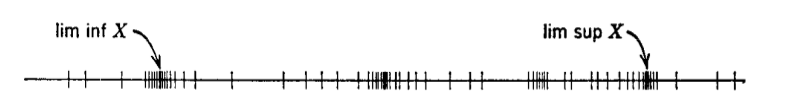
\includegraphics[height=1.5cm]{1_01.png}

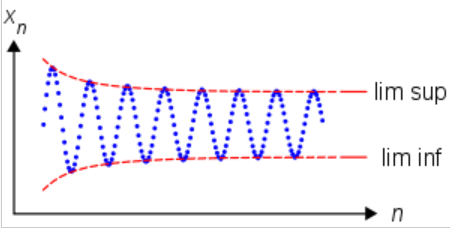
\includegraphics[height=3cm]{1_02.png}

Formel olarak diyelim ki $\{x_n\}$ bir seri, ve diyelim ki bir reel
sayi $S$ var, ki bu reel sayi su sartlari tatmin ediyor 
1) Her $\epsilon > 0$ icin bir $N$ var, oyle ki her $n>N$ icin $x_n
< S + \epsilon$ 
ve 2) her $\epsilon > 0$ ve $M>0$ icin bir  $n>M$ var ki $x_n
> S - \epsilon$. O 
zaman $S$ sayisina  $\{x_n\}$ serisinin limit superior'u denir. 

Bu tanimin soylemeye calistigi serinin yaklastigi degerden sonra ve once
sonlu buyuklukte (bir pencere tanimlarsak bu pencere icinde sonlu sayida
eleman olacaktir (sonsuz degil). Bu pencerenin tanimlanabiliyor olmasi,
onun makul bir noktada olmasini gerektirir, ki bu nokta da yaklasilan
degerden baskasi degildir. 

Limit inferior bunun tersidir, 

\[ \lim \inf x_n  = -\lim \sup(-x_n)\]




















\end{document}
